\documentclass[12pt]{article}
\usepackage[a4paper,width=160mm,top=20mm,bottom=20mm,bindingoffset=6mm]{geometry}
\usepackage[superscript,biblabel]{cite}
\usepackage{graphicx}
\usepackage{caption}
\usepackage{subcaption}

\usepackage{tabularx}


\title{A novel and multipurpose autonomous drone platform}

\date{September 10, 2016}

\author{
	Sundaramahalingam, Sudharshan\\
	\and
	Isaac Tay Eng Hian\\
	\and
	Prahlad Vadakkepat
}

\begin{document}

\maketitle
\pagenumbering{gobble}
\newpage
\pagenumbering{arabic}

\section{Abstract}
The Unmanned Aerial Vehicle (UAV) industry has seen a market growth from 552 million USD to 1.4 billion in a span of a year finding applications in several fields including but not limited to agriculture, security and fire-fighting. Currently, the most common and widely available drone platforms are quadrotors- multicopters which use 4 rotors for flight and steering through the concept of differential thrust to each motor. However, as the drone industry expands to provide drone solutions for niche applications, the quadcopter platforms fall short in terms of accessibility, safety and affordability. This project solves that problem by constructing a novel drone flight platform which enhances the performance of existing drones and allows them to be easily applied to many drone solutions. This task requires the platform to have high modularity in the hardware and software while maintaing high safety standards and affordability. An affordable and open architecture drone, SentiBot, is detailed in this work. SentiBot uses a enclosed dual-propeller design similar to coax-copters like the Spherical Flying Vehicle from Japan while using thrust vectoring for steering. SentiBot's moving parts are enclosed within the frame which enhances safety and it's electronics are mounted on the external recessed surface which enhances electronics accessiblity. It is equipped with a dual-processor CPU, the Intel Edison and the STM32F103, to compartmentalise low-level and high-level computational task which allows greater code modularity and code efficiency. The hardware is built to be fully modular and accessible such that the drone can be multipurpose and adapted to several different drone solutions on demand. The software is built Cleanflight and Robot Operating System (ROS) which are both open-source and highly modular allowing software modularity as well. The drone is equipped with 4 IR sensors and 1 RGB camera for autonomous flight as well. It is able to fly stably and is extremely compact, coming in at 9x9x11cm. It can fly in obstacle filled environments a due to its collision protection shell. SentiBots achieves a 15 minute flight-time with a max payload capacity of 100g. With SentiBots, researchers and inventors are able to use the hardware and software modularity to build several variations of the drone to target niche use-cases. This is in contrast to existing quadrotors which lack the hardware flexibilty and accessibility to be as multipurpose as the SentiBot. In conclusion, we have constructed a fully modular hardware and software platform for drone developers to build a wide range of drone solutions due to the multipurpose and autonomous nature of the drone platform.

\newpage

\section{Introduction}

The Unmanned Aerial Vehicle (UAV), commonly known as a drone, industry has seen a market growth from a 552 million USD industry in 2014, to 1.4 billion USD in 2015 with an expected forecast of 5 billion USD by 2017\cite{legalandsocial}. Drones are being applied to practical uses in agriculture, surveillance, security and industrial automation. One application of drones is a military attack platform where the industry is estimated to reach 1.8 trillion by 2017\cite{dronewars}. Another application is in the agriculture industry through monitoring of crops, large plantations and vegetation\cite{agriculture}. Specialized applications include mosquito vector control\cite{mosquito} and oil spill detection monitoring\cite{oilspill}. 

Quadrotor helicopters or quadcopters are currently the most common drone platforms available. They operate on the mechanics of 4 rotors spinning at varying velocities which allows the drone to achieve steering and thrust through a PID loop based control system\cite{Multiwii}. These quadcopters are unaffordable in large quantities for projects and implementations involving swarm robotics and distributed robotic systems. Quadrotor platforms also have exposed rotors which raises safety concerns for use. Although these platforms have free APIs, the hardware is closed-source making it hard for institutions to develop drone solutions based on quadcopter platforms.

This project seeks to develop a novel drone model which is capable of addressing the safety concerns with existing drone platforms while providing features which allow for easy implementation into several drone solutions. The project also ensures easy development for researchers such that the drone platform be easily modified for deployment into several drone solutions.

An affordable and open architecture drone, namely SentiBot, is detailed in this work. SentiBot utilizes a dual-propeller electronic ducted fan (EDF) with an enclosed frame in a coax-copter design. The design increases safety while decreasing the cost and enables high modularity. The frame is 3D-printed which allows easy hardware replication for experimentation to be conducted with additional sensors. The platform has the Intel Edison System on a Chip (SoC) and a unique dual CPU architecture which enables compartmentalization of computational tasks.\cite{inteledison}The higher level tasks are managed by the Intel Edison CPU while the lower level real-time tasks are handled by the ATMEGA 328 8-bit microcontroller running a real time operating system (RTOS). The platform utilizes Yocto Linux and supports ROS which provides open source libraries and software resources\cite{ROS}. The platform is intended to enhance the operational safety, payload carrying capacity, scalability, performance and affordability of existing drone platforms. The focus of the report is towards the hardware aspect of the drone platform and the software aspect involves minor modifications to existing open-source software to demonstrate flight performance.

\section{SentiBot hardware design}

In this section, the rationale behind the hardware design and the novelty of this design is outlined and explained. Additionally, challenges during the design process and the design methodology used are discussed and the performance of the final drone platform is analyzed in this section.

\subsection{Targets of the drone platform}

The concern with drone safety has resulted in the stringent regulation by governments on the usage of drones in public and in industries. The safety of the drone is thus critical. A lower cost drone platform allows a greater adoption rate by reserachers as budget proves to be less of a concern.\cite{stateschoolfunding} Robotics platforms used in research need to provide easy access to hardware and software systems to enable researchers to change aspects of the platform for specific use cases\cite{materialrobotics}. The three aspects of an ideal drone platform is summarized as safety, affordability and accessibility. 

\subsection{Modular, 3D printed drone frame design}

The Sentibot uses a novel frame design which is made through additive material fabrication using a Nylon-6 filament as Nylon-6 provides a high durability to weight ratio which is favorable for a flying platform\cite{3Dprinting}. The novelty of the design is that the electronics in housed outside of the main body in contrast to the internal housing seen in other coax copters\cite{SFV}. Having the electronics outside the main body enhances the accessibility of the electronics components. 

A modular frame design based on support beams holds the frame together. The frame is designed in a cylindrical form as the compressive strength of cylinders has been shown to be superior of cuboids due to lack of discrete stress points like the corners of a cuboid\cite{cylinderstrength}.A two part motor assembly is used to enclose 2 counter-rotating rotors which creating a ducting effect. The ducting of the motors increases efficiency at high rotary speeds and also enhances the static thrust performance of the system\cite{ductedfan}.

The frame's motor mounting struts were initially flattened on the positive Z-axis which led to air resistance resulting in loss of motor efficiency. The design is improved such that the motor-mounting strut is flattened on the positive X-axis which gives the strength and rigidity of the motor mount while preventing air resistance through the frame.

\begin{figure}
	\centering
	\begin{subfigure}{0.5\textwidth}
		\centering
		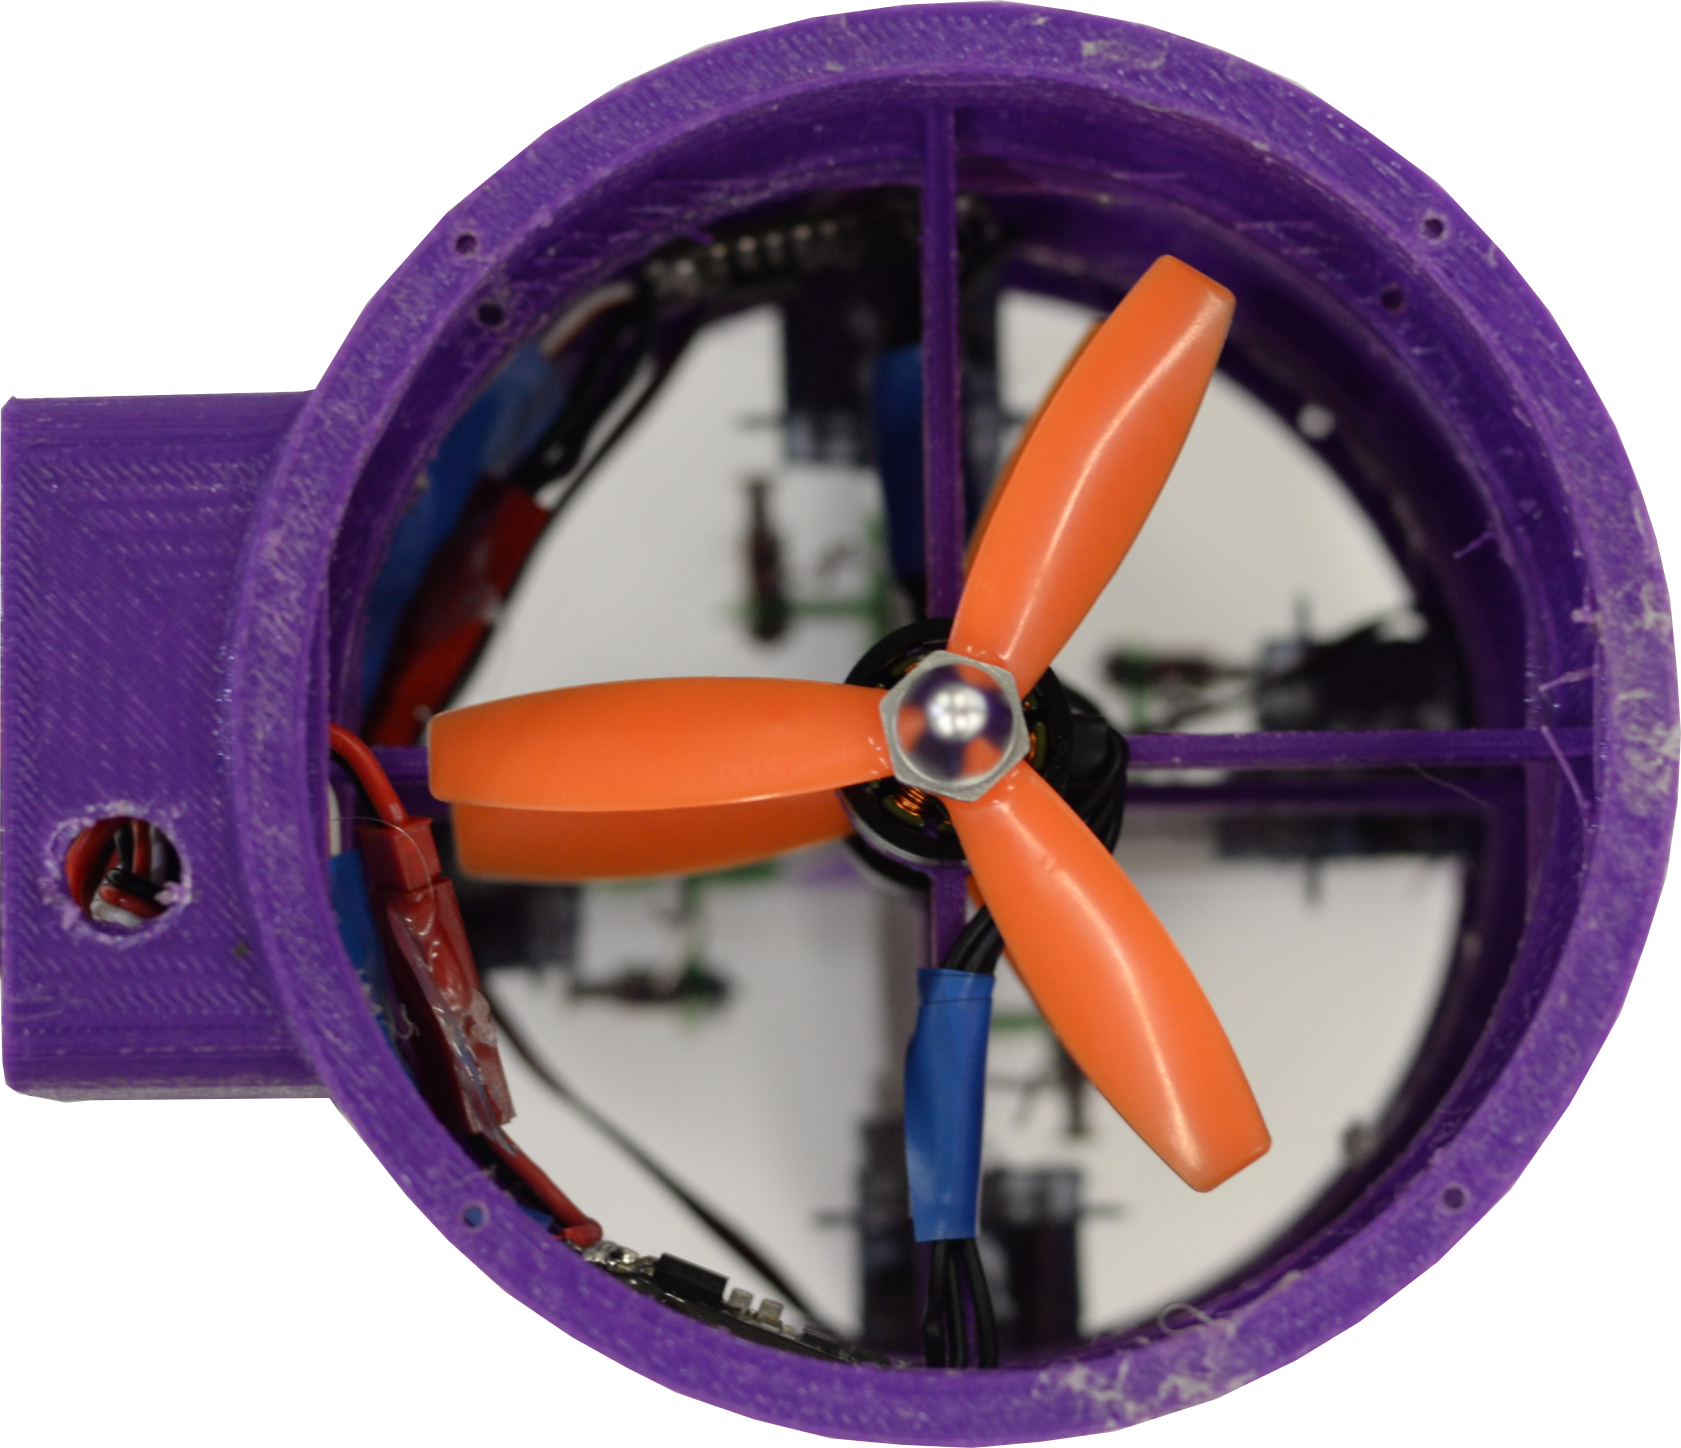
\includegraphics[width=0.9\linewidth]{sb-topdown.png}
		\caption{Top-down view of the SentiBot}
		\label{fig:sb-topdown}
	\end{subfigure}%
	\begin{subfigure}{0.5\textwidth}
		\centering
		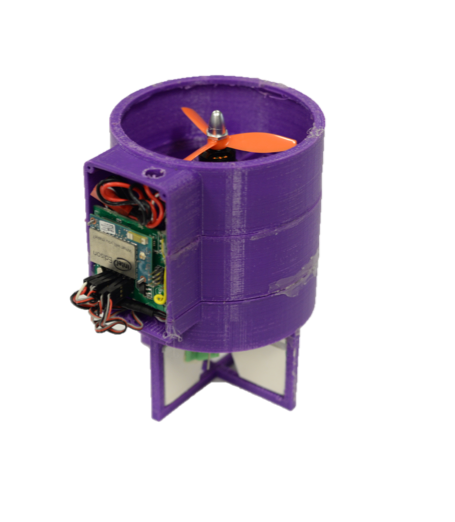
\includegraphics[width=0.9\linewidth]{sb-side.png}
	\caption{Perspective view of the SentiBot}
	\label{fig:sb-side}
	\end{subfigure}
\end{figure}

\subsection{Control system and steering}

Four servos were utilized to control 4 independently movable control surfaces. This 4-servo configuration is found in other coaxial-copters\cite{SFV}. The number of servos have been reduced to two through the coupling of control surfaces on the same axis. Coupling adjacent control surfaces lead to the loss in yaw control, but this was compensated in the introduction of coaxial motors elaborated on later. The control surfaces are made of foam board and are protected by a housing to minimise damage on landing. 

\subsection{Coaxial dual-motor thrust design}

Three motor configurations were considered. Configuration A uses a single 4000 kV electronic ducted fan (EDF).  Configuration B utilizes a single 4000 kV racing quadcopter motor which is drives a 3040 triple blade propeller. Configuration C uses two 4000 kV motors driving the 3040 triple blade propeller stacked vertically with an inter-propeller distance of 8 cm. Configuration C is significant as it accounts for the counter-torque effects produced by the motor and offers a method to cancel the effects unlike the other configurations which require active compensation from the control surfaces.

We tested the configurations by measuring the average thrust output and current consumption of 10 measurements. The results in Table \ref{tab:configs} aproximate the efficiency and maximum thrust output provided by each configuration. Given the battery capacity, flight time expectations and the mass of the SentiBot, the ideal configuration for the SentiBot can be determined.

\begin{table}[h]
	\centering
	\begin{tabular}{ | l | l | l | }
		Configuration & Maximum Thrust/g & Maximum Current/A \\
		\hline
		Single EDF & 200 & 18 \\
		Single motor & 250 & 13 \\
		Stacked motors & 450 & 23 \\
	\end{tabular}
	\caption{Results of the tested configurations}
	\label{tab:configs}
\end{table}

The ideal configuration is determined to be Configuration C and by using counter-rotating bullnose propellers with a 4000kV race quad motor, the SentiBot can achieve a high thrust to space ratio. Performance analysis of rotors show that larger diameter rotors are more efficient as compared to smaller rotors\cite{propellor}. The SentiBot uses 2 large rotors arranged in a stacked configuration as compared to a quadrotor which uses 4 smaller rotors arranged in a plane thus higher efficiency can be obtained from the SentiBot\cite{propellor}. This allows for a compact frame design while preserving the payload carrying capacity.

\subsection{Aerodynamic analysis of the frame}
The frame underwent aerodynamic analysis to determine the efficiency and drag co-efficient of the frame. Through this analysis, the frame can be ensured to be streamlined and to allow for efficient movement during operation. It additionally allows for a higher speed during flight.

\begin{figure}[h]
	\centering
	\begin{subfigure}{0.5\textwidth}
		\centering
		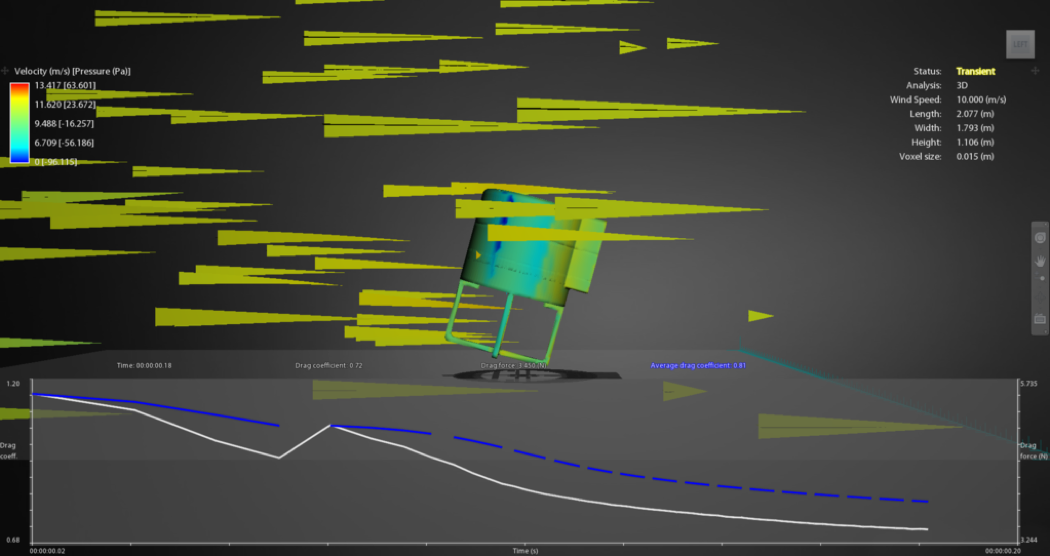
\includegraphics[width=0.9\linewidth]{aerodynamic-1.png}
	\end{subfigure}
	\caption{Screenshots of the aerodynamic analysis}
	\label{fig:aerodynamic}
\end{figure}

The aerodynamic analysis of the frame in Figure \ref{fig:aerodynamic} shows that due to the cylindrical frame design, the body is minimized. During forward motion, the drag primarily arises from the electronics compartment but it is considered negligible as the craft is too small for these effects to manifest in a significant manner. The one-sided nature of the electronics compartment results in the loss of radial symmetry which gives rise to some instability but the software mechanisms have been designed and tuned to compensate for these errors. 

\begin{table}[h]
	\centering
	\begin{tabular}{ | l | l | }
		Component & Hardware \\
		\hline
		Main Processor & Dual core 500Mhz Intel Atom \\
		Secondary Processor & ATMEGA 328 \\
		Motors & 4000KV motors \\
		ESCs & 12A XMS series \\
		Batteries & 800mAh 4S(14.8v) \\
		Propellers & 3x3x4.5 \\
		Servos & 2.8g ultralight \\
		Thrust & 500g \\
		Weight & 250g \\
	\end{tabular}
	\caption{Hardware components of the SentiBot}
	\label{fig:components}
\end{table}

\section{SentiBot Electronics Design}

The electronics of the robot aids in the the robot's ability to function and the accessability of these electronics enhances the learning process of users of concepts invovling electrical engineering and PCB design. The electronics serves as a hardware platform for the software to act upon. In this section, the challenges and solutions to desiging and building a electronics subsystem are outlined and the rationale for our final design is explained.

\subsection{Dual CPU architecture}

A powerful onboard processor is required as computing power intensive tasks cannot be offloaded to a ground-station when certain types of research and experiments like swarm intelligence and decentralized computing\cite{swarm} are being conducted. Vision processing and autonomous navigation also are very computing intensive\cite{vision}. The SentiBot has an Intel Edison System on Chip (SoC) which consists of a 500Mhz Intel Atom, an Intel Quark microcontroller, 1GB of onboard DDR3 RAM and 4GB of onboard flash storage. The onboard processors provide the flexibility of the platform by running Yocto Linux which is a flavour of Linux built for embedded systems and robotics. 

An STM32F103 32-bit microcontroller is used as a secondary processor to provide more General Purpose IO (GPIO) and sensor expandability. A dual-layer PCB is designed to integrate the Intel Edison and the STM32F103 in a dual-CPU architecture. Higher-level tasks are executed in the Intel Edison while time-critical tasks like communication with sensors and actuators are done in the STM32F103. The separation of the higher and lower level processing provides code modularity in the software.

This Dual-CPU architecture was derived from the combination of attributes specific to micro-processors and micro-controllers which provides both the benefits of having a powerful micro-processor (high computing power, Linux based operating system, interfaces like I2S, USB and CAN, fast data movement between various memory locations) and the benefits of having a powerful micro-controller (real-time operation, fast speed of execution, more GPIO). 

\subsection{On board sensors}

The main sensor which allows for the drone to fly in a stable manner is the Inertial Measurement Unit (IMU). The IMU provides accelerometer and gyroscope information to the STM32F103 for the PID loop to keep the drone upright. The sensor also allows for dead reckoning to be used for localization\cite{ultrasonic}.

The IR distance sensors mounted on all 4 sides allows for collision avoidance to prevent crashes. There is also an onboard RGB camera which interfaces to the primary processor over USB. 

\subsection{Flight Drive system specifications}

The power electronics consists of four 1-cell 1200 mAh batteries, two 30 A Electronic Speed Controllers (ESC) and two 4000kV 1306 motors. The motors have a maximum current rating of 8A each and taking into consideration that the maximum thrust of each motor is 370g, the gram per current rating for each motor is 46 g/A. The weight of the SentiBot is about 320g, the nominal current draw during a hover would be about 7A. That gives a flight time of about 10-15 minutes. 

In terms of power management, 3 voltage levels are required - 14.8V from the battery, 5V for the control board and 3.3V for the control circuity. Since the drone’s ESCs do not come equipped with a built in battery eliminator circuit (BEC) an external switching regulator is used to supply clean 5V for the control board. The onboard 3.3V regulator further steps down the voltage from 5V to 3.3V

\begin{figure}[h]
	\centering
	\begin{subfigure}{0.5\textwidth}
		\centering
		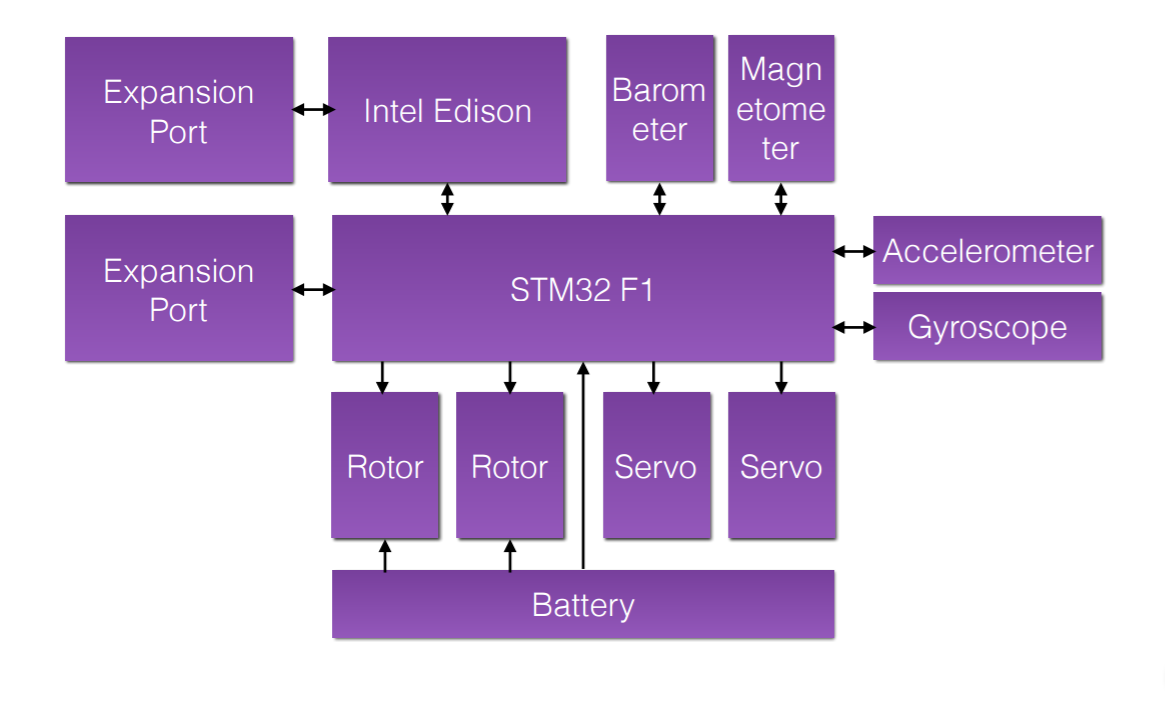
\includegraphics[width=1\linewidth]{framework.png}
	\end{subfigure}
	\caption{Electronics Wireup}
	\label{fig:electronics}
\end{figure}

\section{Software Design}

SentiBots has two methods of operation: manual and autonomous. In manual, an operator has full control and information from the drone. Operated autonomously, the drone is user-programed to complete tasks with little or no human intervention. SentiBots has two subsystems: control and intelligence. The control subsystem consists of the hardware interface to GPIO and the Inertial Measurement Unit (IMU), and relevant Proprotional Integral Derevative (PID) loops. It also can provide basic obstacle avoidance. The intelligence subsystem is for complex tasks like navigation, localization, vision, object identification and other tasks for autonomous flight. It also provides communication with the groundstation.

\subsection{Lower level subsystem}

The control algorithm in SentiBot is standard. Sensor data is mapped into error values that can be used to compensate for frame errors and instabilities. IMU data (processed by an internal Digital Signal Processor) is read over I\textsuperscript{2}C to obtain yaw-pitch-roll (YPR) data. Each YPR value is used in PID loops for each axis to obtain error values. The angle of the control surfaces are set by the error values, therefore stabilizing the system. This computation runs on the ATmega 328.

As shown in figure \ref{fig:intelsystem}, an I\textsuperscript{2}C peripheral interface is used between the lower level subsystem and the IMU. A USART interface is used between the microcontroller and the processor running the higher level subsystem. This communication is managed by software that utilizes the Multi-Wii protocol\cite{SFV}.

The firmware which runs the lower level subsystem is based on the open-source Cleanflight project. Minor modifications were made to the firmware for coax-copter support but the built-in Multi-Wii PID loop controller and communication infrastructure were used. The open-source Cleanflight framework is modular and easy to modify for the end user. The Cleanflight platform is also well documented and easy to understand. The lower level subsystem carries out basic collision avoidance system with 4 IR sensors installed around the bot. This prevents higher level algorithms from allowing crashes and damage to the bot and the environment. This is done through a modification that is made to the Cleanflight framework which adds collision avoidance functionality to it.

\subsection{Higher Level subsystem}

The autonomy of the SentiBots, when implemented in a fully modular manner, allows researchers to tap onto resources available online and libraries for implementing autonomy in the SentiBots for case-specific solutions. Thus, the SentiBots is based on the ROS architecture which is completely open source and provides existing libraries for researchers to easily implement systems into the robots. The ROS architecture is already used by students and researchers.

The communication system is reliant on the onboard WiFi chipset present in the Intel Edison SoC. It connects to an 802.11n network operated by the ground station and transmits over the established network. It also transmits telemetry information gathered from hardware through the microcontroller and sensor expansion port.

\section{Applications}

SentiBots is a multipurpose robotic platform which enhances the performance of current quadcopters for niche applications and implementations. Researchers can use the platform to develop problem-specific solutions using the hardware and software modularity built into the platform. A few of the applications are listed in Table 3 below. Note that this list is non-exhaustive and several other niche problems can be solved with this platform.

\begin{table}[h]
	\centering
	\begin{tabularx}{\linewidth}{ | >{\setlength\hsize{.3\hsize}} X | >{\setlength\hsize{.5\hsize}} X }
		Applications of SentiBot & Description \\
		\hline
		Education & Compact, safe and accessible nature of SentiBot makes it a desirable education drone platform \\
		Agriculture &  Sentibots is smaller and more durable than quadcopters making it ideal for agriculture \\
		Surveillance and Security & SentiBots is small, hard to detect and equipped with a camera for military reconnaisance  \\
		Fire-Fighting & The durability and enclosed electronics makes SentiBots more shielded from fire allowing for drone based fire fighting solutions \\
		Forest Monitoring & SentiBot is small and quiet enough to avoid disturbing wildlife while preventing illegal poaching \\
	\end{tabularx}
	\caption{Proposed lesson plan outline (16-18)}
	\label{tab:lessonplan1}
\end{table}

\section{Results}

The results of testing were positive. The SentiBot shows the ability to lift off, and fly in a stable hover with minimal user intervention. When moved around, the SentiBot platform can accurately maintain its attitude without much user compensation. Furthermore, the drop tests showed that the SentiBot can survive drops from up to 3m high due to its rigid 3D printed Nylon-6 frame. These drop tests were conducted through flying to robot up to a certain height and removing power from the motors and measuring how high we could drop from before there was damage to the frame. 5 test runs was conducted. The top speed achieved from the SentiBot is about 20km/h and flight times are about 15 minutes with normal flying. The SentiBot can achieve versatile flight through, under and over obstacles without collisions due to its small size and form factor. The SentiBot can easily survive collisions with walls or other obstacles without falling due to its shell.

The project has accomplished its goal of designing and constructing a novel drone platform which solves many of the problems with conventional drones. In the future, work can be conducted into some specific use-cases with this drone which allows us to implement the drone platform as a real-life drone solution.

\bibliographystyle{unsrt}
\bibliography{report}

\end{document}
